\documentclass[12pt, openany]{report}
\usepackage[utf8]{inputenc}
\usepackage[T1]{fontenc}
\usepackage{amsmath,amsfonts,amssymb}
\usepackage{amssymb}
\usepackage{multicol}
\usepackage[a4paper,left=2.5cm,right=2.5cm,top=2.5cm,bottom=2.5cm]{geometry}
\usepackage[english]{babel}
\usepackage{libertine}
\usepackage{graphicx}
\usepackage{wrapfig}
\usepackage{algorithm}
\usepackage{algpseudocode}
\usepackage{float}
\usepackage{enumitem}
\usepackage{pythonhighlight}
\usepackage[]{titletoc}
\usepackage{empheq}
\usepackage{titlesec}
\usepackage{mathpazo}
\usepackage{xfrac}
\usepackage{textcomp}
\usepackage{mathtools}
\usepackage{caption}
\usepackage{tabularray}
\usepackage{subcaption}
\usepackage[bottom]{footmisc}
\usepackage{pdfpages}
\usepackage{tabularx}
\usepackage{amsthm}
\usepackage[skins]{tcolorbox}
\titleformat{\chapter}[display]
  {\normalfont\bfseries}{}{0pt}{\Huge}
\usepackage{hyperref}
\newcommand{\hsp}{\hspace{20pt}}
\newcommand{\HRule}{\rule{\linewidth}{0.5mm}}
\newcommand{\R}{\mathbb{R}}
\newcommand{\C}{\mathbb{C}}
\newcommand{\E}{\mathbb{E}}
\theoremstyle{definition}
\newtheorem{thm}{Theorem}[chapter]
\newtheorem{definition}[thm]{Definition}
\newtheorem{lem}[thm]{Lemma}

\hbadness=100000
\begin{document}
\begin{titlepage}
    \begin{sffamily}
    \begin{center}
        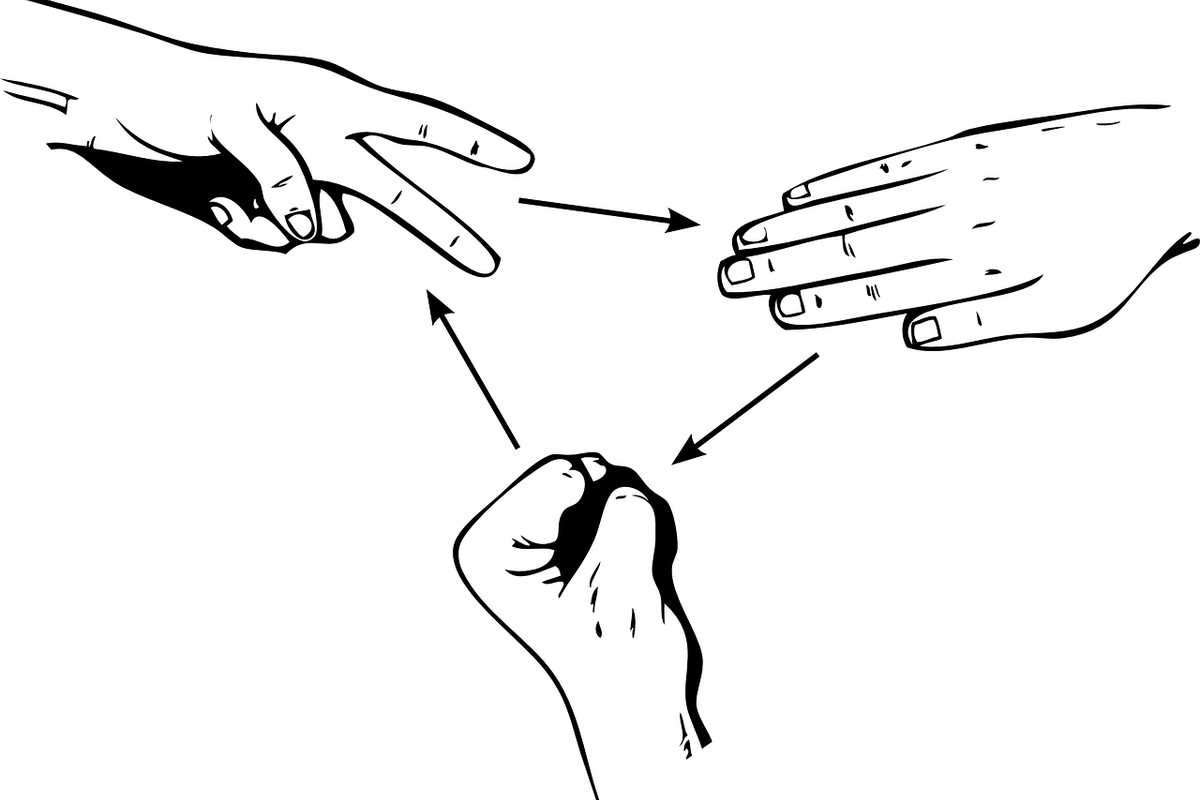
\includegraphics[scale=0.25]{img/page_de_garde.png} \\[1cm]
        \HRule \\[0.4cm]
        { \huge \bfseries LINMA2111 - Discrete mathematics II \\[0.4cm] }
    
        \HRule \\[1.5cm]
        \textsc{\LARGE Simon Desmidt}\\[1cm]
        \vfill
        \vspace{2cm}
        {\large Academic year 2025-2026 - Q1}
        \vspace{0.4cm}
         
        
\includegraphics[width=0.15\textwidth]{img/epl.png}
        
        UCLouvain\\
    
    \end{center}
    \end{sffamily}
\end{titlepage}

\setcounter{tocdepth}{1}
\tableofcontents
\chapter{We will see}
\section{Sorting problem}
\subsection{Introduction}
A sorting problem is a problem that consists of taking a sequence of $n$ objects and putting them in order. This kind of problem is made of three main elements:
\begin{itemize}
  \item Context: set $S$ with a partial order $<$;
  \item Input: $n$ elements of $S$;
  \item Output: permutation of the input elements respecting the order.
\end{itemize}
To prove the correctness of an algorithm, we generally use the Hoare triple, i.e. a tuple for any input array $x_0$:
\begin{equation}
  \begin{aligned}
	&\{\text{Algorithm to be used};\ \text{Precondition}; \ \text{post condition}\}\\
	&\left\{IS;\ x=x_0;\ x\text{ is sorted and is a permutation of }x_0\right\}
\end{aligned}
\end{equation}
where IS is the insertion sort algorithm, and $x$ is the sorted array. From now on, we will call "sorting" a sorted permutation. \\
In practice, to prove the correctness of an algorithm, we define the invariant and the base case, and do an induction step show that the invariant is preserved.\\
\subsection{Complexity}
\textcolor{red}{Add the slide on complexity.}
We define the average case complexity as an expectation of the time taken by the algorithm on each input possible, with a dependence in the size of the input.
\begin{equation}
	t = \mathbb{E}_{x\sim D}[T(x)]
\end{equation}
where $D$ is the distribution of the input.\\
\subsection{Divide and conquer}
The divide and conquer method consists in three steps:
\begin{enumerate}
	\item Divide: create smaller subproblems;
	\item Recurse: solve them;
	\item Combine: merge the solutions.
\end{enumerate}
In sorting problems, a divide-and-conquer algorithm is the merge sort algorithm. It consists in dividing the array in two, sorting each half recursively, and merging the two sorted halves. The merge operation is done in linear time.\\
\end{document}